\section{Asymptotics of the exterior parametrix}
By using the summation formula derived in LV12 the existence and values of the
asymptotic components of the specific operator we're looking at can be
calculated directly. From Lemma bla we know, that we only have to consider $j\in
\{0, 1, 2\}$ since the requested asymptotic coefficient is of order $-5$.

\subsection{Preliminaries}
In (%größtenteils)
accordance with LV12 we denote
\begin{align*}
    % TODO Anständig einführen im Setting, Unterschiede zum LV12-paper ausweisen
    % TODO Explizit darauf hinweisen, dass alle gewöhnlichen Funktionen als
    %      Multiplikationsoperator zu verstehen sind.
    % TODO Es ist gesteigert eklig, dass R_+ negatives Vorzeichen hat …
    R_- &:= \Eto{-\mu\left|x-y\right|} \\
    R_+ &:= -C(\mu,\theta)\Eto{-\mu(x+y)} \\
    R_\theta &:= \tfrac1{2\mu} (R_- + R_+) \\
    R_{(\sigma_1,\sigma_2,\ldots,\sigma_n)} &:= 
    \left(\tfrac1{2\mu}\right)^n R_{\sigma_1} \lambda(V,W) R_{\sigma_2} \dots
    \lambda(V,W) R_{\sigma_n} \\
    R^{(j)} &:= (-1)^j \psi \left( [R_\theta \lambda(V,W)]^j R_\theta -
    [R_\mathbb{R}\lambda(V,W)]^j R_\mathbb{R}\right) \phi \\
            &= (-1)^j
                \sum_{
                        \substack{
                         \sigma\in\{+,-\}^j \\
                         \sigma\neq(+,\ldots,+)
                         }
                        }
                     \psi R_\sigma
                \phi
\end{align*}

We also set
\begin{align}
    \Lambda(x) := \Integ[x]{0}{t}{\lambda(t)}\quad\text{and}\quad
    \mathrm M(x) := \Integ[x]{0}{t}{\Lambda(t)}.
\end{align}

We will need both of the following Lemmas for the calculation. The first one is
a classical result of asymptotic analysis and is the base of all further results
on the asymptotics of exponential integrals.
\begin{Lemma}[Watson]
    Let $\phi\colon [0,1] \to \mathbb{C}, \phi(t) = t^\sigma g(t)$ such that $g$ is
analytic in some neighbourhood of $t=0$, $\sigma > -1$, $\beta > 0$, and
\begin{equation*}
    \exists_{C, b > 0} \forall_{t > 0} \left|\phi(t)\right| < C \Eto{bt}.
\end{equation*}
Then the exponential integral
\begin{align*}
    F(x) := \Integ[T]{0}{t}{\Eto{-\beta\,xt}\phi(t)}
\end{align*}
is finite for all $x \geq 0$ and has the asymptotic expansion in terms of the
gamma function $\Gamma$ (see Appendix~\ref{app:gamma})
\begin{equation*}
    F(x)\SimAs{x\to\infty}\sum_{n=0}^{\infty}
    \frac{g^{(n)}(0)}{(\beta x)^{n+\sigma+1}} \frac{\Gamma(n+\sigma+1)}{n!}
\end{equation*}

    \begin{proof}
        Since the proof is a bit lengthy and not needed to understand the
        following it can be found in Appendix~\ref{sec:proof-watson}.
    \end{proof}
%    \begin{Remark}
%        We actually don't need analyticity but only the existence of as many
%        derivatives as degrees we want and additionally a finiteness condition
%        on .
%    \end{Remark}
\end{Lemma}

The second Lemma is a quite general formula for nested integrals, in which the
upper limit of the inner integral is the integration variable of the outer one:
\begin{Lemma}
    \label{lem:triangle-integration}
    Let $f,g\colon[0,1]\to\mathbb{R}$ be continuous. Then the following formula
    holds:
    \begin{align*}
        \Integ[1]{0}{x}{g(x)\Integ[1]{x}{y}{f(y)}} =
        \Integ[1]{0}{y}{f(y)\Integ[y]{0}{x}{g(x)}}
    \end{align*}
    \begin{proof}
        Let $F(x) := \Integ[x]{0}{y}{f(y)}$ and $G(y) := \Integ[y]{0}{x}{g(x)}$.
        Then we see using partial integration:
        \begin{align*}
            \Integ[1]{0}{x}{g(x)\Integ[1]{x}{y}{f(y)}} &=
            \Integ[1]{0}{x}{g(x)F(1)} - \Integ[1]{0}{x}{g(x)F(x)} \\
            &= G(1)F(1) - \left(\Bigl.G(y)F(y)\Bigr|_0^1 -
            \Integ[1]{0}{y}{G(y)f(y)}\right) \\
            &= \Integ[1]{0}{y}{G(y)f(y)} =
            \Integ[1]{0}{y}{f(y)\Integ[y]{0}{x}{g(x)}},
        \end{align*}
        which proves the given formula.
    \end{proof}
    \begin{Remark}
      The special case $f\equiv g$ results in the formula
      \begin{align*}
        \Integ[1]{0}{x}{f(x)\Integ[1]{x}{y}{f(y)}} = 
        \Integ[1]{0}{y}{f(y)\Integ[y]{0}{x}{f(x)}} = 
        \frac12 F(1)^2.
      \end{align*}
    \end{Remark}
\end{Lemma}

\begin{Remark}
  This is in fact only Fubini's theorem for the integral of $(x,y)\to g(x)f(y)$
  over a right-angled triangle:
  \begin{center}
    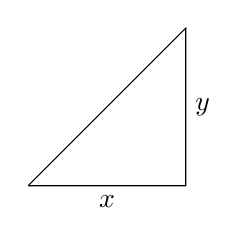
\begin{tikzpicture}
      \draw (0,0)
      -- (2,2)
      -- node[anchor=west] {$y$} (2,0)
      -- node[anchor=north] {$x$} (0,0);
    \end{tikzpicture}
  \end{center}
\end{Remark}

With those given we can explicitly calculate the asymptotics of the
resolvent-trace. 

\subsection{Calculations}
% TODO
From the above considerations we know that we will have to calculate the
asymptotics of $2^3 - 1 + 2^2 - 1 + 2^1 - 1 = 11$ traces. For symmetry reasons
we can reduce this to 7 integrals.
% TODO: Symmetrieüberlegungen! Das muss gehen (denn es funktioniert), ist aber
% nichttrivial. Sind die Integrale stetig in x und y? Das ist quasi der wichtige
% Punkt. Ist F(x) = \int e^(-tx) f(t) stetig? Sollte es sein, genau an diese
% Stelle gehört der zugehörige Beweis.

% TODO: Achtung: Für Lipschitzstetigkeit braucht man offenbar \int tf(t),
% nachsehen, ob das hier gegeben ist. Wenn nicht, nochmal mit einfacher
% Stetigkeit probieren.
\begin{Lemma}
  Let $f\colon [0,T)\to\mathbb{R}$ (where $T$ can be $\infty$) be an integrable
    function. Then the exponential integral
  \begin{align*}
    F(x) = \Integ[T]{0}{t}{\Eto{-tx} f(t)}
  \end{align*}
  is continuous in $x$.
  \begin{proof}
    We only need the Lipschitz continuity of the exponential function for
    negative exponents:
    \begin{align*}
      \lvert F(x) - F(y)\rvert &=
      \left|\Integ[T]{0}{t}{\Eto{-tx}f(t)} - \Integ[T]{0}{t}{\Eto{-ty}f(t)}\right|
      = \left|\Integ[T]{0}{t}{\left(\Eto{-tx}-\Eto{-ty}\right)f(t)}\right| \\
      &\le \Integ[T]{0}{t}{L\left|x - y\right| \lvert tf(t)\rvert}
      = L \left\|f\right\|_{L^1([0,T))} \left|x-y\right|,
    \end{align*}
    where $L$ is the Lipschitz constant for $x\mapsto\exp(-x)$ on $\Rplus$.
  \end{proof}
\end{Lemma}

In the following calculations we define $C := \frac{C(\mu,\theta)}{2\mu} \to
-(2\mu)^{-1}$ as $\mu\to\infty$.

The calculation for $j=0$ is straightforward:
\begin{align}
  \Tr R^{(0)} &= \Int{x}{k_\theta(x,x;\mu) - k_\mathbb{R}(x,x;\mu)} \\
              &= -C \Int{x}{\Eto{-2\mu x}} \\
              &= -C \left(
                \frac1{2\mu} - \frac{\Eto{-2\mu}}{2\mu}
                \right) \\
              &\SimAs{\mu\to\infty}\ -\frac1{4\mu^2}
  \label{eqn:jeq0}
\end{align}

For $j=1$ and $j=2$ we need to employ both Watson's Lemma and our integration
formula.

% TODO: Sichergehen, dass wenigstens j=1 schonmal stimmt!
% j = 1, ++
The first term for $j=1$ is as follows
\begin{align*}
  \Tr R^{(1)}_{++} &= C^2 \Int{x}{
    \Int{z}{
      \Eto{-\mu(x+z+z+x)}\lambda(z)
    }
  } \\
  &= C^2 \Int{x}{
    \Eto{-2\mu x}
  }
  \Int{z}{
    \Eto{-2\mu z}\lambda(z)
  } \\
  &= C^2 \left(
      \frac1{2\mu} - \frac{\Eto{-2\mu}}{2\mu}
    \right)
    \Int{z}{\Eto{-2\mu z}\lambda(z)} \\
  &\SimAs{\mu\to\infty}\ %
  \frac{1}{2\mu} \Wsum{\lambda^{(n)}(0)}
\end{align*}

% j = 1, +-
The second term for $j=1$ is
\begin{align*}
  \Tr R^{(1)}_{+-} &= -C^2 \Int{x}{
      \Int{z}{
        \Eto{-\mu(x+z+\Abs{z-x})}
        \lambda(z)
      }
    } \\
    &= -C^2 \Int{x}{
      \left(
        \Integ[x]{0}{z}{
          \Eto{-\mu(x+z+x-z)}\lambda(z)
        }
      + \Integ[1]{x}{z}{
          \Eto{-\mu(x+z-x+z)} \lambda(z)
        }
      \right)
    } \\
    &= -C^2 \left(
      \Int{x}{\Eto{-2\mu x} \Lambda(x)}
      + \Int{x}{\Eto{-2\mu x} \lambda(x)x}
      \right) \\
      % Result:
    &\SimAs{\mu\to\infty}\ %
      -\frac{1}{2\mu}
      \Wsum{\Lambda^{(n)}(0)} + \Wsum{n\lambda^{(n-1)}(0)} \\
      %
    &= \Wsum{(n+1)\lambda^{(n-1)}},
\end{align*}
since $\Lambda(0) = 0$. We also used the identity $(xf(x))^{(n)} = xf^{(n)}(x) +
nf^{(n-1)}(x)$ as well as the triangle integration
(Lemma~\ref{lem:triangle-integration}) with $g \equiv 1$.
% j = 1, -+
For the symmetry reasons given above this does also give the asymptotics of $\Tr
R^{(1)}_{-+}$.

% j = 2
The calculations for $j = 2$ are a bit more involved. Again, we need to
transform the integrals such that we can apply Watson's lemma. The least
problematic term is again the one without any absolute values in the exponent:
% TODO: Falsch gerechnet :), Vorzeichen!
% +++
\begin{align*}
  \Tr R^{(2)}_{+++} &= C^3
  \Int{x}{
    \Int{z_1}{
      \Int{z_2}{
        \Eto{-\mu(x + z_1 + z_1 + z_2 + z_2 + x)}
        \lambda(z_1)\lambda(z_2)
      }
    }
  } \\
  &= C^3 \Int{x}{
    \Eto{-2\mu x}
  }
  \left(
    \Int{z}{
      \Eto{-2\mu z}\lambda(z)
    }
  \right)^2 \\
  % Result
  &\SimAs{\mu\to\infty}\ %
  \frac{1}{(2\mu)^6}
  \left((2\mu)\Wsum{\lambda^{(n)}(0)}\right)^2
\end{align*}

Now we calculate the case $\Tr R^{(2)}_{++-} =  \Tr R^{(2)}_{-++}$ as follows
\begin{align*}
  \Tr R^{(2)}_{-++} &= -C^3 \Int{x}{
    \Int{z_1}{
      \Int{z_2}{
        \Eto{-\mu(\Abs{x-z_1} + z_1 + z_2 + z_2 + x)}
        \lambda(z_1)\lambda(z_2)
      }
    }
  } 
  % TODO: Nicht fertig, war falsch
\end{align*}
Very similar to that we can calculate $\Tr R_{+-+}$:
% +-+
\begin{align*}
  \Tr R_{+-+}^{(2)} &= -C^3 \Int{x}{
    \Int{z_1}{
      \Int{z_2}{
        \Eto{-\mu(x+z_1 + \lvert z_1 - z_2\rvert + z_2 + x)}
        \lambda(z_1)\lambda(z_2)
      }
    }
  } \\
  &= -C^3 \Int{x}{
    \Eto{-2\mu x} \left(
      \Int{z_1}{
        \Integ[1]{z_1}{z_2}{
          \Eto{-\mu(2z_2)}\lambda(z_1)\lambda(z_2)
        }
        + \Integ[z_1]{0}{z_2}{
          \Eto{-\mu(2z_1)}\lambda(z_1)\lambda(z_2)
        }
      }
    \right)
  } \\
  &= -C^3 \Int{x}{\Eto{-2\mu x}}
    \Int{z}{
      \Eto{-2\mu z}\left(
        \Lambda(z)\lambda(z) + z (\lambda(z))^2
      \right)
    }
\end{align*}

\begin{align*}
  \Tr R_{--+}^{(2)} &= C^3 \Int{x}{
    \Int{z_2}{
      \Int{z_1}{
        \Eto{-\mu(\Abs{x-z_1} + \Abs{z_1 - z_2} + z_2 + x)}
        \lambda(z_1)\lambda(z_2)
      }
    }
  } \\
  &= C^3 \Int{x}{
    \left(
      \Integ[x]{0}{z_2}{
        \left(
          \Integ[z_2]{0}{z_1}{
            \Eto{-2\mu(x + z_2 - z_1)}\lambda(z_1)\lambda(z_2)
          }
          + \Integ[1]{z_2}{z_1}{
            \Eto{-2\mu(x)}\lambda(z_1)\lambda(z_2)
          }
        \right)
      } \\
    &\hphantom{=} + \Integ[1]{x}{z_2}{
        \left(
          \Integ[z_2]{0}{z_1}{
            \Eto{-2\mu z_2}\lambda(z_1)\lambda(z_2)
          }
          + \Integ[1]{z_2}{z_1}{
            \Eto{-2\mu z_1}\lambda(z_1)\lambda(z_2)
          }
        \right)
      }
    \right)
  }
\end{align*}
% 
% TODO:
% Das habe ich auch noch nicht zuende gerechnet!

% -+-
\begin{align*}
  \Tr R_{-+-}^{(2)} &= C^3 \Int{x}{
    \Int{z_2}{
      \Int{z_1}{
        \Eto{-\mu(\Abs{x-z_1}+z_1+z_2+\Abs{z_2-x})}\lambda(z_1)\lambda(z_2)
      }
    }
  } \\
  &= C^3 \Int{x}{
    \Eto{-2\mu x}
    \left(
      \Lambda(x)^2 + \lambda(x)M(x) + \ldots
      % TODO: Dritter Term ist noch nicht 
      % gerechnet!
    \right)
  }
\end{align*}

Now that we have calculated all those terms we only need to sum them up and
match coefficients to get the first three terms in the asymptotic expansion of
$\Tr(\Delta_\lambda + z^2)^{-1}$. In particular we have to deal with the fact,
that $\lambda(x) = \lambda^2 V(x) + W(x)$ is of mixed order. Furthermore we note
that, as it was for the interior parametrix, the coefficients of the trace
expansion are again a homogeneous polynomial in $V$, $W$ and their respective
derivatives. Assuming that we can carry on with our method (which is possible
though highly tedious) this will also hold for higher orders, since it will by
construction only produce positive integer powers of $\lambda(x)$ and its
derivatives.
% TODO: PROOF, das ist wichtig (sagt Lesch!)
%       Annahme dazu: Wir können jedes Integral der Art \Tr R_{+-+-+-+…}^{(n)}
%       in eine Form bringen, so dass Watson's Lemma angewandt werden kann.

Summing up the previous results we get the following three terms of the
asymptotic expansion of $\Tr R_\theta$:
% TODO: Achtung: Hier ist nicht verwendet, dass \lambda = \lambda^2 V + W, also
%       von gemischter Ordnung ist! Außerdem muss \mu = \sqrt(\lambda^2 + z^2)  
%       ausgeschrieben werden
\begin{align}
  h_1 &= \frac{1}{4\mu^2} = \frac{1}{4} (\lambda^2 + z^2)^{-1} \\
  h_2 &= \frac{1}{8\mu^3} (\lambda'(0) + 6\lambda'(0)) =
         \frac{7}{8\mu^3}\lambda'(0) \\
  h_3 &= 
\end{align}

